\section{Относительность движения}

\begin{ex}
Два поезда движутся навстречу друг другу со скоростью $v$ каждый. 
Определите время встречи поездов, если начальное расстояние между ними равно $L$. 
Решите задачу координатным способом, графическим способом и методом, использующим идею относительности движения.
\begin{ans}
$\frac{L}{2v}$
\end{ans}
\end{ex}

\begin{ex}
Муха летает между двумя сближающимися со скоростью $v$ стенками. 
Скорость мухи $u$. Начальное расстояние между стенками равно $L$. 
Какой путь пройдет муха до остановки, если считать, что как только она приближается к одной из стенок -- мгновенно изменяет 
направление скорости на противоположное и движется вдоль одной прямой, перпендикулярной стенкам?
\begin{ans}
$\frac{uL}{v}$
\end{ans}
\end{ex}

\begin{ex}
Проплывая под мостом против течения, гребец потерял соломенную шляпу. Обнаружив пропажу через десять минут, он повернул назад и, гребя с тем же темпом, подобрал шляпу на расстоянии 900 м ниже моста. 
Через какое время после обнаружения пропажи гребец подобрал шляпу?
\begin{ans}
10 мин
\end{ans}
\end{ex}

\begin{ex}
(2012)\footnote{Здесь и далее год в скобках означает, что данная задача была предложена для решения на Краевой студенческой олимпиаде по физике в Пермском крае в указанном году.}
Когда мимо пристани проплывает плот, от пристани в деревню, расположенную на расстоянии $S$ вниз по течению реки, отправляется моторная лодка. Она доходит до деревни за время $t$ и, сразу повернув обратно, встречает плот на расстоянии $ S_1 $ от деревни. Какова скорость течения реки $\vec{v}_p$?
\begin{ans}
$v_p = (S - S_1)/t$
\end{ans}
\end{ex}

\begin{ex}
С какой скоростью $\vec u$ должен двигаться автомобиль, чтобы капли дождя не оставляли следов на заднем стекле, наклоненном под углом $ \alpha $? Скорость дождя $\vec v$.
\begin{ans}
$u > v / \tan \alpha$
\end{ans}
\end{ex}

\begin{ex}
Открытая карусель вращается с угловой скоростью $\omega $. На карусели на расстоянии $r$ от оси вращения стоит человек. 
Идет дождь, и капли дождя падают вертикально вниз со скоростью $v_0$. 
Как человек должен держать зонт, чтобы наилучшим образом укрыться от дождя?
\begin{ans}
Под углом $\alpha$ к вертикали, $\tan \alpha = \omega r / v_0$
\end{ans}
\end{ex}

\begin{ex}
(2009) Самолет в безветренную погоду взлетает со скоростью $\vec v$  под углом к горизонту $\alpha_0$. Внезапно начинает дуть горизонтальный встречный ветер, скорость которого $\vec u$. Какой стала скорость самолета относительно земли $w$, и какой угол $\alpha$ составляет она с горизонтом?
\begin{ans}
$w = \sqrt{v^2 + u^2 - 2uv\cos \alpha_0}$,
$\alpha = \alpha_0 + \arcsin \left( \frac{u}{w} \sin \alpha \right)$
\end{ans}
\end{ex}

\begin{ex}
(2013) Самолет садится на корабль, движущийся по океану со скоростью $\vec{v}_1$ в восточном направлении. 
Скорость ветра $\vec{v}_2$ направлена на север, а самолет снижается по отношению к кораблю вертикально со скоростью $\vec{v}_3$. 
Определить величину скорости самолета по отношению к движущемуся воздуху.
\begin{ans}
$\vec{v} = \vec{v}_1 + \vec{v}_3 - \vec{v}_2$, 
$v = \sqrt{v_1^2 + v_2^2 + v_3^2}$, 
\end{ans}
\end{ex}

\begin{ex}
Под каким углом к направлению течения должен плыть пловец, 
чтобы переправиться на противоположный берег с наименьшим смещением из-за течения реки? 
Скорость пловца $\vec u$, скорость реки $\vec v$.
\begin{ans}
$\cos \alpha = v/u, u > v$, либо $\cos \alpha = u/v, u < v$
\end{ans}
\end{ex}

\begin{ex}
Шарик движется навстречу стенке со скорость $\vec u$, скорость движения стенки $\vec v$. 
Определите, с какой скоростью отскочит шарик от стенки после абсолютно упругого удара. 
Как изменится ответ, если стенка движется в ту же строну, что и шарик? 
Если шарик падает под углом $ \alpha $ к стенке?
\begin{ans}
$u + 2v$
\end{ans}
\end{ex}

\begin{ex}
Определите кратчайшее расстояние между автомобилями, которые движутся со скоростями $v$ по перпендикулярным пересекающимся прямым. 
В начальный момент времени один автомобиль находится в центре перекрестка, а второй подъезжает к нему на расстоянии $L$. 
Как изменится ответ, если угол между прямыми равен $\alpha$?
\begin{ans}
$L/\sqrt{2}$
\end{ans}
\end{ex}

\begin{ex}
Как изменяется расстояние между двумя каплями воды, которые свободно падают в поле силы тяжести? 
Обе капли выпущены из одной точки с интервалом времени $\tau = 1$ с.
\begin{ans}
$g \tau t + g \tau^2 / 2$
\end{ans}
\end{ex}

\begin{ex}
Два тела движутся по прямой навстречу друг другу с начальными скоростями $\vec{v}_1$ и $\vec{v}_2$ и 
постоянными ускорениями $\vec{a}_1$ и $\vec{a}_2$, направленными противоположно соответствующим скоростям в начальный момент времени. 
При каком максимальном начальном расстоянии $L_{\max}$ между телами они встретятся в процессе движения?
\begin{ans}
$L_{\max} = \frac{(v_1 + v_2)^2}{2(a_1+a_2)}$
\end{ans}
\end{ex}

\begin{ex}
От колеса радиуса $R$, движущегося без проскальзывания по горизонтальной поверхности со скоростью $\vec v$,  отрывается вертикально кусочек грязи и, пролетев по воздуху, возвращается точно в ту же точку, от которой оторвался. При каких условиях это возможно?
\begin{ans}
$v^2 = \pi g R n$, где $n \in \mathbb{N}$
\end{ans}
\end{ex}

\begin{ex}
\hspace{0pt} \\
\begin{minipage}{.65\textwidth}
Два колечка $O$ и $O'$ надеты на вертикальные неподвижные стержни $AB$ и $A'B'$ соответственно. 
Нерастяжимая нить закреплена в точке $A'$ и на колечке $O$ и продета через  колечко $O'$. 
Считая, что колечко $O'$ движется вниз с постоянной скоростью $\vec{v}_1$, определите скорость $\vec{v}_2$ колечка $O$, если  $\angle AOO' = \alpha$.
\end{minipage}
\begin{minipage}{.35\textwidth}
\centering
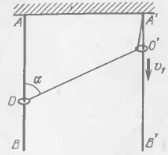
\includegraphics[width=0.9\textwidth]{0113RelativityRings.jpg}
\end{minipage}
\begin{sol}
Перейдем в систему отсчета, связанную с колечком $O'$. В этой системе отсчета скорость точки $O$ равна $v_1/ \cos \alpha$ и направлена вверх, так как нить нерастяжима и относительно колечка $O'$ веревка выбирается с постоянной скоростью $v_1$. Поэтому относительно прямой $АА'$, связанной с землей, скорость колечка $O$ будет равна $v_2 = \frac{v_1}{\cos \alpha} - v_1 = v_1 \frac{\sin^2 (\alpha /2)}{\cos \alpha}$ и направлена вверх.
\end{sol}
\begin{ans}
$v_2 = v_1 \frac{\sin^2 (\alpha /2)}{\cos \alpha}$
\end{ans}
\end{ex}

\begin{ex}
\hspace{0pt} \\
\begin{minipage}{.65\textwidth}
На неподвижном клине, образующем угол $\alpha$  с горизонтом, лежит нерастяжимая невесомая веревка. Один из концов веревки прикреплен к стене в точке $A$. В точке $B$ к веревке прикреплен небольшой грузик. В некоторый момент времени клин начинает двигаться вправо с постоянным ускорением $\vec{a}$. Определите ускорение $\vec{a}_2$ грузика, пока он находится на клине.
\end{minipage}
\begin{minipage}{.35\textwidth}
\centering
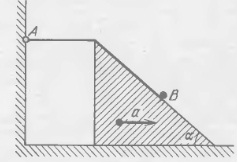
\includegraphics[width=0.9\textwidth]{0114RelativityWedge.jpg}
\end{minipage}
\begin{sol}
К моменту времени $t$ от начала движения клин пройдет расстояние $s = at^2/2$ и приобретет скорость $v_1 = at$. За это время грузик переместится вдоль клина на такое же расстояние $s$, а его скорость относительно клина будет равна $v_2 = at$ и направлена вдоль клина вверх. Скорость грузика относительно земли равна $\vec{v}_3 = \vec{v}_1 + \vec{v}_2$. Поскольку угол между векторами $\vec{v}_1$ и $\vec{v}_2$ равен $\alpha$, то $v_3 = 2at \sin (\alpha /2)$. \\ 
Угол, который скорость $\vec{v}_3$ составляет с горизонтом, равен $\beta  = (\pi - \alpha)/2$. Таким образом, грузик движется вдоль прямой, составляющей с горизонтом угол $\beta$ c ускорением $a_2 = 2a \sin (\alpha /2)$.
\end{sol}
\begin{ans}
Ускорение грузика относительно земли $a_2 = 2a \sin (\alpha /2)$ направлено под углом $\beta  = (\pi - \alpha)/2$ к горизонту.
\end{ans}
\end{ex}

\begin{ex}
\hspace{0pt} \\
\begin{minipage}{.65\textwidth}
(2011) По шоссе со скоростью $\vec{v}_a$ движется автобус. Человек находится на расстоянии $h$ от шоссе и на расстоянии $L$ от автобуса. 
Под каким углом $\alpha$ к шоссе со скоростью $\vec v$  должен идти человек, чтобы выйти на шоссе одновременно с автобусом?
\end{minipage}
\begin{minipage}{.35\textwidth}
\centering
\includestandalone[width=0.9\textwidth]{Pictures/012011RelativityBus}
\end{minipage}
\begin{ans}
При $v_a > vL/h$ человек ни при каком угле не сможет оказаться на шоссе раньше автобуса. При $v_a < vL/h$ существует два ответа $\alpha_1 = \arcsin \frac{h}{L} + \arcsin \frac{v_ah}{vL}$ и $\alpha_2 = \pi - \alpha_1$.
\end{ans}
\end{ex}

\begin{ex}
\hspace{0pt} \\
\begin{minipage}{.65\textwidth}
(2007) Два катера вышли одновременно из пунктов $A$ и $B$, находящихся на противоположных берегах реки, и двигались вдоль отрезка $AB$ длины~$l$. 
Прямая $AB$ образует угол $\alpha$ с направлением скорости течения $\vec v$. Скорости движения катеров относительно воды одинаковы. 
На каком расстоянии от пункта $B$ произошла встреча катеров, если они встретились через время $t$ после отхода от причалов?
\end{minipage}
\begin{minipage}{.35\textwidth}
\centering
\includestandalone[width=0.9\textwidth]{Pictures/0115RelativityPowerboats}
\end{minipage}
\begin{ans}
$l/2 - vt \cos \alpha$
\end{ans}
\end{ex}
